\section{Observation}
\begin{table}[h!]\centering\setstretch{1.5}
\begin{tabular}{|l||c|c|} \hline
	\textbf{Mapping} & $\fullfunction{\psi_p}{\Z}{\Z_p}{n}{n\bmod p=\psi_p(n)}$ & $\fullfunction{\phi_a}{\C[x]}{\C}{f(x)}{f(a)=\phi_a(f(x))}$ \\ \hline\hline
	Additive Homo. & $\psi_p(a+b):=(a+b)\bmod p$ & $\phi_a(f+g):=f(a)+g(a)$ \\ \hline
	Multiplicative Homo. & $\psi_p(ab):=(ab)\bmod p$ & $\phi_a(fg):=f(a)g(a)$ \\ \hline
	Kernel & $\ker(\psi_p)=p\Z$ & $\ker(\phi_a)=(x-a)\C[x]$ \\ \hline
	Image & $\Z_p$ & $\C$ \\ \hline
	Ideal & $p\Z=\generate{p}$ & $(x-a)\C[x]=\generate{x-a}$ \\ \hline
	Prime Ideal & $\generate{p}$ is prime & $\generate{x-a}$ is prime \\ \hline
	Maximal Ideal & $\generate{p}$ is maximal & $\generate{x-a}$ is maximal \\ \hline
	Isomorphism & $\Z_p\simeq \Z/p\Z$ & $\C\simeq \C[x]/\generate{x-a}$ \\ \hline
\end{tabular}
\end{table}

\thmbox{\begin{theorem}
Every ideal $I$ of ring $R$ is the kernel of some ring homomorphism.
\end{theorem}}
\begin{proof}
	Let $I$ is an ideal in a ring $R$, that is, $I$ is a subset of $R$ that satisfies: \begin{itemize}
		\item 
	\end{itemize}
\end{proof}
\newpage

\section*{Non-Commutative Rings Without Unity and Prime Ideals}

\subsection*{Example 1: The Ring of 2x2 Upper Triangular Matrices Over a Field \( \mathbb{F} \)}

Consider the ring \( R \) of 2x2 upper triangular matrices over a field \( \mathbb{F} \):

\[
R = \left\{ \begin{pmatrix}
	a & b \\
	0 & c
\end{pmatrix} \mid a, b, c \in \mathbb{F} \right\}
\]

This ring is non-commutative and does not have a unity element.

\subsubsection*{Prime Ideal}

An ideal \( P \) in \( R \) can be the set of matrices where the (1,2)-entry is zero:

\[
P = \left\{ \begin{pmatrix}
	a & 0 \\
	0 & c
\end{pmatrix} \mid a, c \in \mathbb{F} \right\}
\]

To see why \( P \) is a prime ideal, consider matrices \( A \) and \( B \) in \( R \). If the product \( AB \in P \), then the (1,2)-entry of \( AB \) must be zero. This means either the (1,2)-entry of \( A \) is zero or the (1,2)-entry of \( B \) is zero, implying \( A \in P \) or \( B \in P \). Thus, \( P \) is a prime ideal.

\subsection*{Example 2: The Ring of Polynomials in Two Non-commuting Variables Over a Field \( \mathbb{F} \)}

Consider the ring \( R = \mathbb{F}\langle x, y \rangle \), the ring of polynomials in two non-commuting variables \( x \) and \( y \) over a field \( \mathbb{F} \).

\subsubsection*{Prime Ideal}

An ideal \( P \) in \( R \) can be generated by the commutator \( [x, y] = xy - yx \):

\[
P = (xy - yx)
\]

To see why \( P \) is a prime ideal, consider two polynomials \( f \) and \( g \) in \( R \). If \( fg \in P \), then \( fg \) can be written as a multiple of \( xy - yx \). If \( xy - yx \) divides \( fg \), then either \( xy - yx \) divides \( f \) or \( xy - yx \) divides \( g \), meaning \( f \in P \) or \( g \in P \). Thus, \( P \) is a prime ideal.


\newpage
\section*{Proof: Existence of a Basis for Any Vector Space using Zorn's Lemma}

\textbf{Theorem:} Every vector space \(V\) over a field \(F\) has a basis.

\textbf{Proof:} To prove this, we will use Zorn's Lemma, which states:
\begin{quote}
	If every chain (totally ordered subset) of a partially ordered set \(S\) has an upper bound in \(S\), then \(S\) contains at least one maximal element.
\end{quote}

\begin{enumerate}
	\item \textbf{Set Construction:}
	Define the set \(\mathcal{C}\) to be the collection of all linearly independent subsets of \(V\):
	\[
	\mathcal{C} = \{ S \subseteq V \mid S \text{ is linearly independent} \}
	\]
	
	\item \textbf{Partial Order:}
	Partially order \(\mathcal{C}\) by inclusion: \(S \leq T\) if \(S \subseteq T\).
	
	\item \textbf{Chain:}
	Let \(\mathcal{A}\) be a chain in \(\mathcal{C}\). This means that every pair of elements in \(\mathcal{A}\) is comparable under \(\subseteq\). For each pair \(S, T \in \mathcal{A}\), either \(S \subseteq T\) or \(T \subseteq S\).
	
	\item \textbf{Upper Bound for Chain:}
	Define \(U = \bigcup_{S \in \mathcal{A}} S\). We claim that \(U \in \mathcal{C}\), i.e., \(U\) is a linearly independent subset of \(V\).
	\begin{itemize}
		\item Suppose for contradiction that \(U\) is not linearly independent. Then there exists a finite subset \(\{u_1, u_2, \ldots, u_n\} \subseteq U\) and scalars \(a_1, a_2, \ldots, a_n \in F\), not all zero, such that:
		\[
		a_1 u_1 + a_2 u_2 + \cdots + a_n u_n = 0
		\]
		\item Each \(u_i\) belongs to some \(S_i \in \mathcal{A}\), and since \(\mathcal{A}\) is a chain, there exists an \(S \in \mathcal{A}\) such that \(u_1, u_2, \ldots, u_n \in S\).
		\item But \(S\) is linearly independent, so the only solution to this linear combination is \(a_1 = a_2 = \cdots = a_n = 0\), a contradiction.
	\end{itemize}
	Thus, \(U\) must be linearly independent, and \(U \in \mathcal{C}\) is an upper bound for the chain \(\mathcal{A}\).
	
	\item \textbf{Application of Zorn's Lemma:}
	By Zorn's Lemma, \(\mathcal{C}\) contains a maximal element \(B\).
	
	\item \textbf{Maximal Linearly Independent Set:}
	Let \(B\) be a maximal element in \(\mathcal{C}\). We claim that \(B\) is a basis for \(V\).
	\begin{itemize}
		\item \(B\) is linearly independent by construction.
		\item Suppose \(B\) is not a basis for \(V\). Then there exists some vector \(v \in V \setminus \text{span}(B)\). The set \(B \cup \{v\}\) would then be linearly independent (otherwise \(v\) would be in the span of \(B\)), contradicting the maximality of \(B\).
	\end{itemize}
	
	\item \textbf{Conclusion:}
	Therefore, \(B\) must span \(V\), making \(B\) a basis for \(V\).
\end{enumerate}
\newpage
\section*{Proof: Co-Finite Topology is a Topology}

\textbf{Definition:} The co-finite topology on a set \(X\) is defined as follows: a subset \(U \subseteq X\) is open if and only if \(U = \emptyset\) or \(X \setminus U\) is finite.

\textbf{Proof:} We need to show that the co-finite topology on \(X\) satisfies the three properties of a topology:

\begin{enumerate}
	\item \(X\) and \(\emptyset\) are in the topology.
	\item The topology is closed under arbitrary unions.
	\item The topology is closed under finite intersections.
\end{enumerate}

\subsection*{1. \(X\) and \(\emptyset\) are in the topology}
\begin{itemize}
	\item \(X\) is open because \(X \setminus X = \emptyset\), which is finite.
	\item \(\emptyset\) is open by definition.
\end{itemize}

\subsection*{2. Closed under Arbitrary Unions}

Let \(\{ U_i \}_{i \in I}\) be an arbitrary collection of open sets in the co-finite topology. We need to show that \(U = \bigcup_{i \in I} U_i\) is open.

\begin{itemize}
	\item If any \(U_i = X\), then \(U = X\), which is open.
	\item If all \(U_i \neq X\), then \(X \setminus U_i\) is finite for each \(i\).
\end{itemize}

Consider \(U = \bigcup_{i \in I} U_i\). Then:
\[ X \setminus U = X \setminus \left( \bigcup_{i \in I} U_i \right) = \bigcap_{i \in I} (X \setminus U_i). \]

Since each \(X \setminus U_i\) is finite, the intersection of any collection of finite sets is finite (or empty). Therefore, \(X \setminus U\) is finite, which implies \(U\) is open in the co-finite topology.

\subsection*{3. Closed under Finite Intersections}

Let \(U_1, U_2, \ldots, U_n\) be a finite collection of open sets in the co-finite topology. We need to show that \(U = \bigcap_{i=1}^n U_i\) is open.

\begin{itemize}
	\item If any \(U_i = X\), then \(U = \bigcap_{i=1}^n U_i = \bigcap_{j \neq i} U_j\), reducing the problem to fewer sets.
	\item If all \(U_i \neq X\), then each \(X \setminus U_i\) is finite.
\end{itemize}

Consider \(U = \bigcap_{i=1}^n U_i\). Then:
\[ X \setminus U = X \setminus \left( \bigcap_{i=1}^n U_i \right) = \bigcup_{i=1}^n (X \setminus U_i). \]

Since each \(X \setminus U_i\) is finite, the union of a finite number of finite sets is finite. Therefore, \(X \setminus U\) is finite, which implies \(U\) is open in the co-finite topology.

\textbf{Conclusion:} Since the co-finite topology on \(X\) satisfies the three properties required for a topology, it is indeed a topology.

\section*{Proof: Zero Sets of Polynomials Form a Co-Finite Topology}

\textbf{Definition:} The zero set of a polynomial \(p \in \mathbb{C}[x]\) is \(Z(p) = \{ z \in \mathbb{C} \mid p(z) = 0 \}\).

\textbf{Proof:} We need to show that the collection of zero sets of polynomials in \(\mathbb{C}\) forms the closed sets of the co-finite topology on \(\mathbb{C}\).

\subsection*{1. Zero Sets are Closed in the Co-Finite Topology}

Let \(p(x) \in \mathbb{C}[x]\) be a non-constant polynomial of degree \(n\). By the Fundamental Theorem of Algebra, \(p(x)\) has at most \(n\) roots in \(\mathbb{C}\). Therefore, \(Z(p)\) is finite.

The zero set of the constant polynomial \(p(x) = 0\) is \(\mathbb{C}\), which is the entire set.

\subsection*{2. Co-Finite Topology Closed Sets}

The closed sets in the co-finite topology are those whose complements are finite. That is, a set \(C \subseteq \mathbb{C}\) is closed if \(\mathbb{C} \setminus C\) is finite or \(C = \mathbb{C}\).

\subsection*{3. Correspondence of Zero Sets and Closed Sets}

\begin{itemize}
	\item The zero set of a non-constant polynomial is finite, corresponding to finite closed sets in the co-finite topology.
	\item The zero set of the constant polynomial \(p(x) = 0\) is \(\mathbb{C}\), corresponding to \(\mathbb{C}\) itself being a closed set in the co-finite topology.
\end{itemize}

\subsection*{4. Characterization of Closed Sets}

To show that the closed sets in the co-finite topology are precisely the zero sets of polynomials, consider:
\begin{itemize}
	\item A finite set \(\{z_1, z_2, \ldots, z_n\}\). This can be written as the zero set of the polynomial
	\[
	p(x) = (x - z_1)(x - z_2) \cdots (x - z_n).
	\]
	\item The whole set \(\mathbb{C}\) is the zero set of the polynomial \(p(x) = 0\).
\end{itemize}

\textbf{Conclusion:} The closed sets in the co-finite topology on \(\mathbb{C}\) are exactly the zero sets of polynomials in \(\mathbb{C}[x]\). Therefore, the collection of zero sets of polynomials forms the closed sets of the co-finite topology, showing that the zero sets of polynomials generate the co-finite topology on \(\mathbb{C}\).

\newpage

\begin{tikzpicture}
	% Draw the open ball
	\draw[thick, dotted] (0,0) circle (2);
	\fill (0,0) circle (0.05) node[below right] {$z_0$};
	\node at (0,-2.3) {Open Ball $B(z_0, r)$};
	\node at (2.3,0) {$r$};
	% Draw radius line
	\draw[<->] (0,0) -- (2,0);
\end{tikzpicture}

%\begin{tikzpicture}
%	% Draw the complex plane as a rectangle
%	\draw[thick] (-3,-2) rectangle (3,2);
%	\node at (0,2.3) {Complex Plane $\mathbb{C}$};
%	
%	% Place zero set points (roots of polynomial)
%	\fill (1,0.5) circle (0.05) node[above] {$z_1$};
%	\fill (-1,-0.5) circle (0.05) node[below] {$z_2$};
%	\fill (0,-1.5) circle (0.05) node[below] {$z_3$};
%	
%	% Label the zero set
%	\node at (0,-2.3) {Zero Set $Z(P)$};
%\end{tikzpicture}
%
%\begin{tikzpicture}
%	% Draw the complex plane as a rectangle
%	\draw[thick] (-3,-2) rectangle (3,2);
%	\node at (0,2.3) {Complex Plane $\mathbb{C}$};
%	
%	% Illustrate a finite set
%	\fill (-2,1) circle (0.05) node[above left] {$z_1$};
%	\fill (2,-1.5) circle (0.05) node[below right] {$z_2$};
%	\fill (0,0) circle (0.05) node[below left] {$z_3$};
%	\fill (1.5,0.5) circle (0.05) node[above right] {$z_4$};
%	
%	% Label finite set and its complement
%	\node at (0,-2.3) {Finite Set in Cofinite Topology};
%	\node at (0,-2.8) {Complement is Infinite};
%\end{tikzpicture}

\newpage


Hence, every vector space \(V\) over a field \(F\) has a basis, as guaranteed by Zorn's Lemma.

\[
\C[x]/\generate{x-\alpha}=
\C[x]/(x-\alpha)\C[x]\simeq\C.
\] Let $f,g\in I=\C[x]/(x-\alpha)\C[x]$. Then \[
f(x)=(x-\alpha)q_1(x) + r(x), q(x)=(x-\alpha)q_2(x) + r(x)
\] Then \[
f(x)\equiv g(x)\pmod{(x-\alpha)\C[x]}\iff f(x)-g(x)\in(x-\alpha)\C[x]
\]
\begin{tikzpicture}
	\begin{axis}[
		axis lines = middle,
		xlabel = {$a$},
		ylabel = {$b$},
		zlabel = {$c$},
		grid = major,
		view = {120}{30},
		width = 10cm,
		height = 8cm,
		samples=10,
		domain=-2:2,
		y domain=-2:2,
		zmin=-2, zmax=2,
		xtick = {-2, -1, 0, 1, 2},
		ytick = {-2, -1, 0, 1, 2},
		ztick = {-2, -1, 0, 1, 2}
		]
		\addplot3[
		scatter,
		scatter src=z,
		only marks,
		mark=*, 
		color=blue,
		opacity=0.5,
		]
		coordinates {
			(1, 0.5, -1.5)
			(1.2, -0.5, 1.8)
			(-1, 0.5, 1)
			(-1.5, -1, 0)
			(0.8, -0.3, 1.2)
		};
	\end{axis}
\end{tikzpicture}
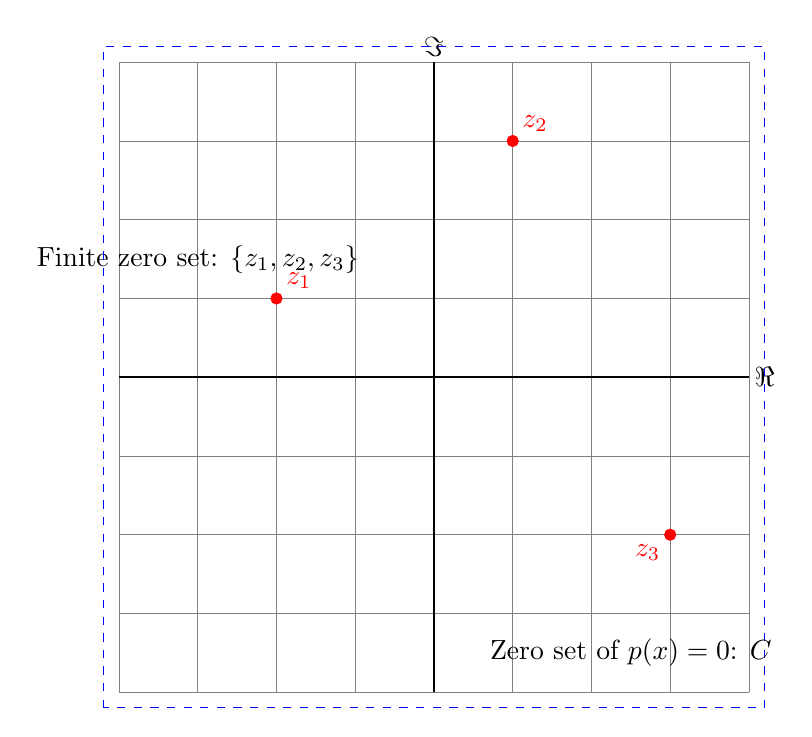
\begin{tikzpicture}
	
	% Draw the complex plane as a rectangle
	\draw[very thin, gray] (-4, -4) grid (4, 4);
	\draw[thick] (-4, 0) -- (4, 0); % Real axis
	\draw[thick] (0, -4) -- (0, 4); % Imaginary axis
	
	% Label the axes
	\node at (4.2, 0) {$\Re$};
	\node at (0, 4.2) {$\Im$};
	
	% Draw some points representing finite zero sets
	\filldraw[red] (-2, 1) circle (2pt) node[above right] {$z_1$};
	\filldraw[red] (1, 3) circle (2pt) node[above right] {$z_2$};
	\filldraw[red] (3, -2) circle (2pt) node[below left] {$z_3$};
	
	% Annotate the points
	\node at (-3, 1.5) {Finite zero set: $\{z_1, z_2, z_3\}$};
	
	% Draw a box around the entire plane representing the zero set of p(x) = 0
	\draw[dashed, blue] (-4.2, -4.2) rectangle (4.2, 4.2);
	\node at (2.5, -3.5) {Zero set of $p(x) = 0$: $\mathbb{C}$};
	
\end{tikzpicture}
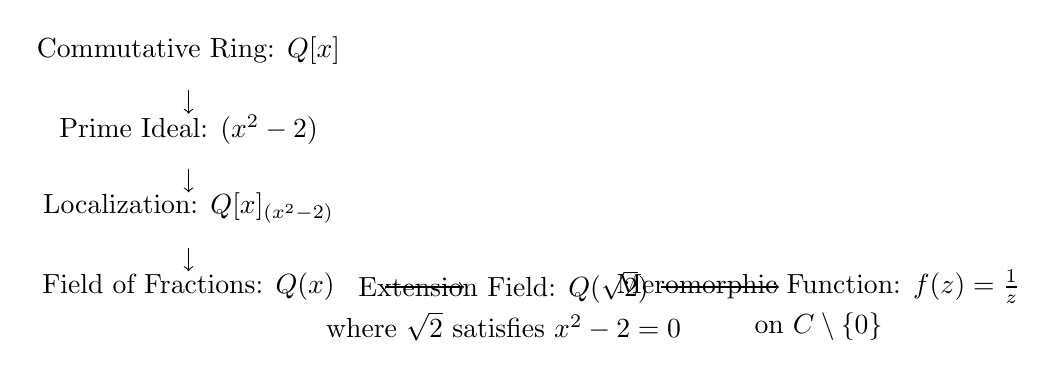
\begin{tikzpicture}
	% Commutative Ring
	\node at (0,4) {Commutative Ring: $\mathbb{Q}[x]$};
	
	% Prime Ideal
	\node at (0,3) {Prime Ideal: $(x^2 - 2)$};
	\draw[->] (0,3.5) -- (0,3.2);
	
	% Localization
	\node at (0,2) {Localization: $\mathbb{Q}[x]_{(x^2-2)}$};
	\draw[->] (0,2.5) -- (0,2.2);
	
	% Field of Fractions
	\node at (0,1) {Field of Fractions: $\mathbb{Q}(x)$};
	\draw[->] (0,1.5) -- (0,1.2);
	
	% Extension Field
	\node at (4,1) {Extension Field: $\mathbb{Q}(\sqrt{2})$};
	\node at (4,0.5) {where $\sqrt{2}$ satisfies $x^2 - 2 = 0$};
	\draw[->] (2.5,1) -- (3.5,1);
	
	% Meromorphic Function
	\node at (8,1) {Meromorphic Function: $f(z) = \frac{1}{z}$};
	\node at (8,0.5) {on $\mathbb{C} \setminus \{0\}$};
	\draw[->] (6,1) -- (7.5,1);
\end{tikzpicture}

\begin{tikzpicture}[scale=1.2]
	% Nodes
	\node (C[x]) at (0,2) {$\mathbb{C}[x]$};
	\node (C) at (4,2) {$\mathbb{C}$};
	\node (poly) at (0,0) {$\alpha(x) = x^2 + 2x + 1$};
	\node (eval) at (4,0) {$\alpha(1) = 4$};
	
	% Arrows
	\draw[->] (C[x]) -- (C) node[midway, above] {$f(\alpha) = \alpha(a)$};
	\draw[->] (poly) -- (eval) node[midway, above] {at $a=1$};
	
	% Coordinate system
	\draw[->] (0,-1) -- (1,-1) node[right] {$x$};
	\draw[->] (0,-1) -- (0,1) node[above] {$y$};
	\draw[domain=-1.5:1.5,smooth,variable=\x,blue] plot ({\x},{\x*\x + 2*\x + 1});
	\fill[red] (1,4) circle (2pt);
	\node at (1.2,4.2) {$(1,4)$};
\end{tikzpicture}

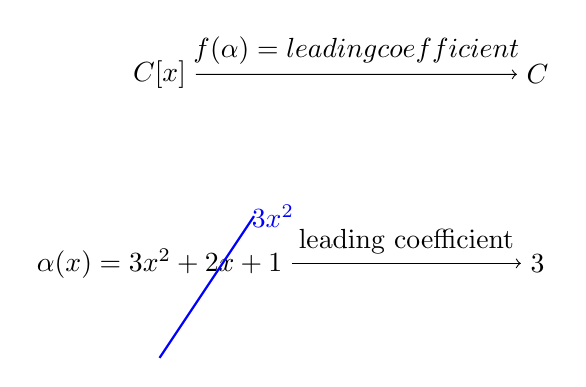
\begin{tikzpicture}[scale=1.2]
	% Nodes
	\node (C[x]) at (0,2) {$\mathbb{C}[x]$};
	\node (C) at (4,2) {$\mathbb{C}$};
	\node (poly) at (0,0) {$\alpha(x) = 3x^2 + 2x + 1$};
	\node (lead) at (4,0) {$3$};
	
	% Arrows
	\draw[->] (C[x]) -- (C) node[midway, above] {$f(\alpha) = \text{leading coefficient}$};
	\draw[->] (poly) -- (lead) node[midway, above] {leading coefficient};
	
	% Illustration
	\draw[thick,blue] (0,-1) -- (1,0.5);
	\node[blue] at (1.2,0.5) {$3x^2$};
\end{tikzpicture}

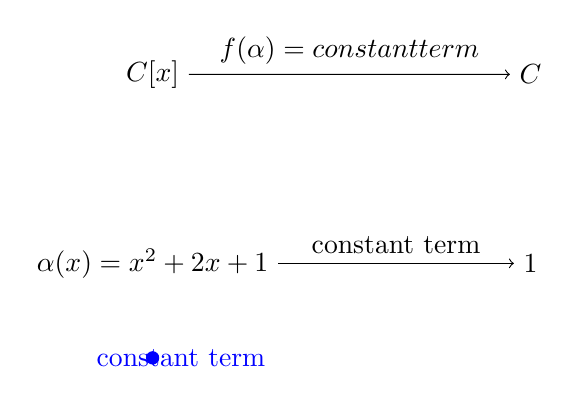
\begin{tikzpicture}[scale=1.2]
	% Nodes
	\node (C[x]) at (0,2) {$\mathbb{C}[x]$};
	\node (C) at (4,2) {$\mathbb{C}$};
	\node (poly) at (0,0) {$\alpha(x) = x^2 + 2x + 1$};
	\node (const) at (4,0) {$1$};
	
	% Arrows
	\draw[->] (C[x]) -- (C) node[midway, above] {$f(\alpha) = \text{constant term}$};
	\draw[->] (poly) -- (const) node[midway, above] {constant term};
	
	% Illustration
	\fill[blue] (0,-1) circle (2pt);
	\node[blue] at (0.3,-1) {constant term};
\end{tikzpicture}

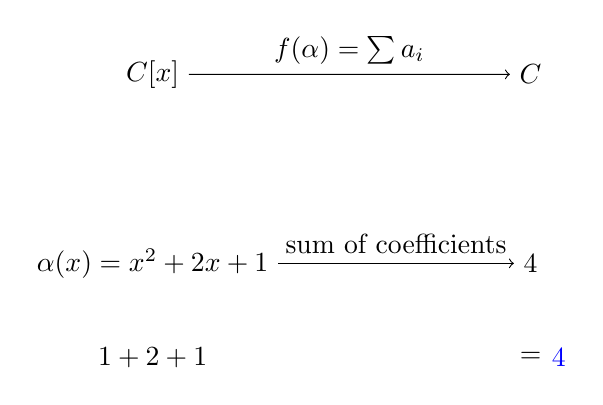
\begin{tikzpicture}[scale=1.2]
	% Nodes
	\node (C[x]) at (0,2) {$\mathbb{C}[x]$};
	\node (C) at (4,2) {$\mathbb{C}$};
	\node (poly) at (0,0) {$\alpha(x) = x^2 + 2x + 1$};
	\node (sum) at (4,0) {$4$};
	
	% Arrows
	\draw[->] (C[x]) -- (C) node[midway, above] {$f(\alpha) = \sum a_i$};
	\draw[->] (poly) -- (sum) node[midway, above] {sum of coefficients};
	
	% Illustration
	\node at (0,-1) {$1 + 2 + 1$};
	\node at (4,-1) {$=$};
	\node[blue] at (4.3,-1) {$4$};
\end{tikzpicture}

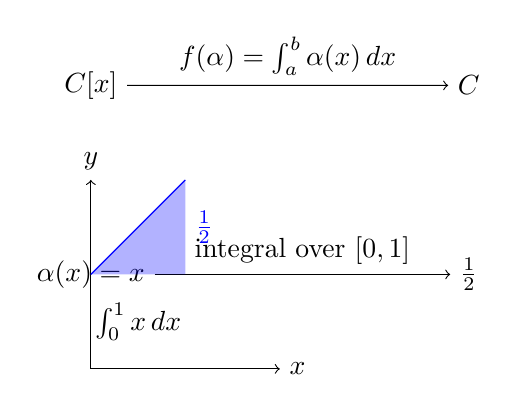
\begin{tikzpicture}[scale=1.2]
	% Nodes
	\node (C[x]) at (0,2) {$\mathbb{C}[x]$};
	\node (C) at (4,2) {$\mathbb{C}$};
	\node (poly) at (0,0) {$\alpha(x) = x$};
	\node (integral) at (4,0) {$\frac{1}{2}$};
	
	% Arrows
	\draw[->] (C[x]) -- (C) node[midway, above] {$f(\alpha) = \int_a^b \alpha(x) \, dx$};
	\draw[->] (poly) -- (integral) node[midway, above] {integral over $[0,1]$};
	
	% Coordinate system
	\draw[->] (0,-1) -- (2,-1) node[right] {$x$};
	\draw[->] (0,-1) -- (0,1) node[above] {$y$};
	\draw[domain=0:1,smooth,variable=\x,blue] plot ({\x},{\x});
	\fill[blue,opacity=0.3] (0,0) -- (1,1) -- (1,0) -- cycle;
	\node at (0.5,-0.5) {$\int_0^1 x \, dx$};
	\node[blue] at (1.2,0.5) {$\frac{1}{2}$};
\end{tikzpicture}

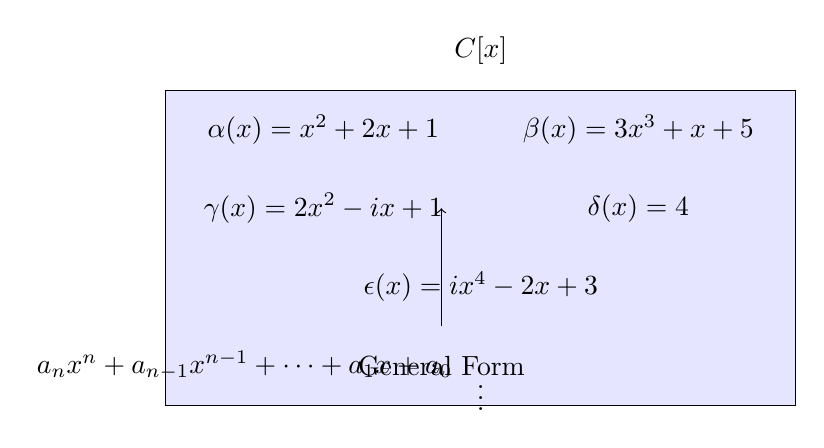
\begin{tikzpicture}
	% Background rectangle for the set
	\draw[fill=blue!10] (0,0) rectangle (8,4);
	\node at (4,4.5) {$\mathbb{C}[x]$};
	
	% Examples of polynomials
	\node at (2,3.5) {$\alpha(x) = x^2 + 2x + 1$};
	\node at (6,3.5) {$\beta(x) = 3x^3 + x + 5$};
	\node at (2,2.5) {$\gamma(x) = 2x^2 - i x + 1$};
	\node at (6,2.5) {$\delta(x) = 4$};
	\node at (4,1.5) {$\epsilon(x) = ix^4 - 2x + 3$};
	
	% Labels and arrows
	\node at (1,0.5) {$a_n x^n + a_{n-1} x^{n-1} + \cdots + a_1 x + a_0$};
	\draw[->] (3.5,1) -- (3.5,2.5);
	\node at (3.5,0.5) {General Form};
	
	% Ellipsis to show continuation
	\node at (4,0.2) {$\vdots$};
\end{tikzpicture}

\begin{tikzpicture}
	% Basis vectors
	\node (1) at (0,0) {$1$};
	\node (x) at (2,0) {$x$};
	\node (x2) at (4,0) {$x^2$};
	\node (x3) at (6,0) {$x^3$};
	\node (dots) at (8,0) {$\cdots$};
	
	% Brackets for vector space
%	\draw[decorate,decoration={brace,amplitude=10pt,mirror}] (-0.5,-0.5) -- (8.5,-0.5);
	\node at (4,-1) {Basis of $\mathbb{C}[x]$};
	
	% Vector space arrow
	\node at (4,-2) {Vector Space $\mathbb{C}[x]$};
	\draw[->] (4,-1.5) -- (4,-2.5);
\end{tikzpicture}

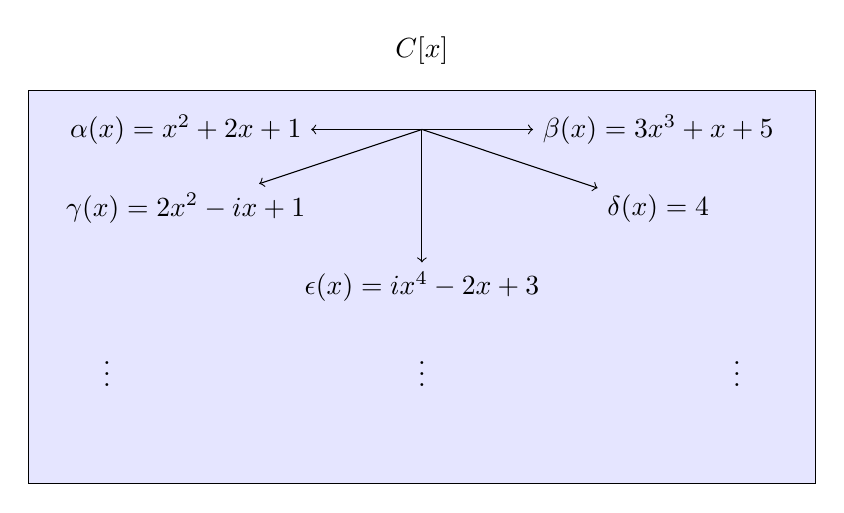
\begin{tikzpicture}
	% Set boundary
	\draw[fill=blue!10] (0,0) rectangle (10,5);
	\node at (5,5.5) {$\mathbb{C}[x]$};
	
	% Examples of polynomials
	\node (alpha) at (2,4.5) {$\alpha(x) = x^2 + 2x + 1$};
	\node (beta) at (8,4.5) {$\beta(x) = 3x^3 + x + 5$};
	\node (gamma) at (2,3.5) {$\gamma(x) = 2x^2 - i x + 1$};
	\node (delta) at (8,3.5) {$\delta(x) = 4$};
	\node (epsilon) at (5,2.5) {$\epsilon(x) = ix^4 - 2x + 3$};
	
	% Connecting lines
	\draw[->] (5,4.5) -- (alpha);
	\draw[->] (5,4.5) -- (beta);
	\draw[->] (5,4.5) -- (gamma);
	\draw[->] (5,4.5) -- (delta);
	\draw[->] (5,4.5) -- (epsilon);
	
	% Set elements
	\node at (1,1.5) {$\vdots$};
	\node at (5,1.5) {$\vdots$};
	\node at (9,1.5) {$\vdots$};
\end{tikzpicture}

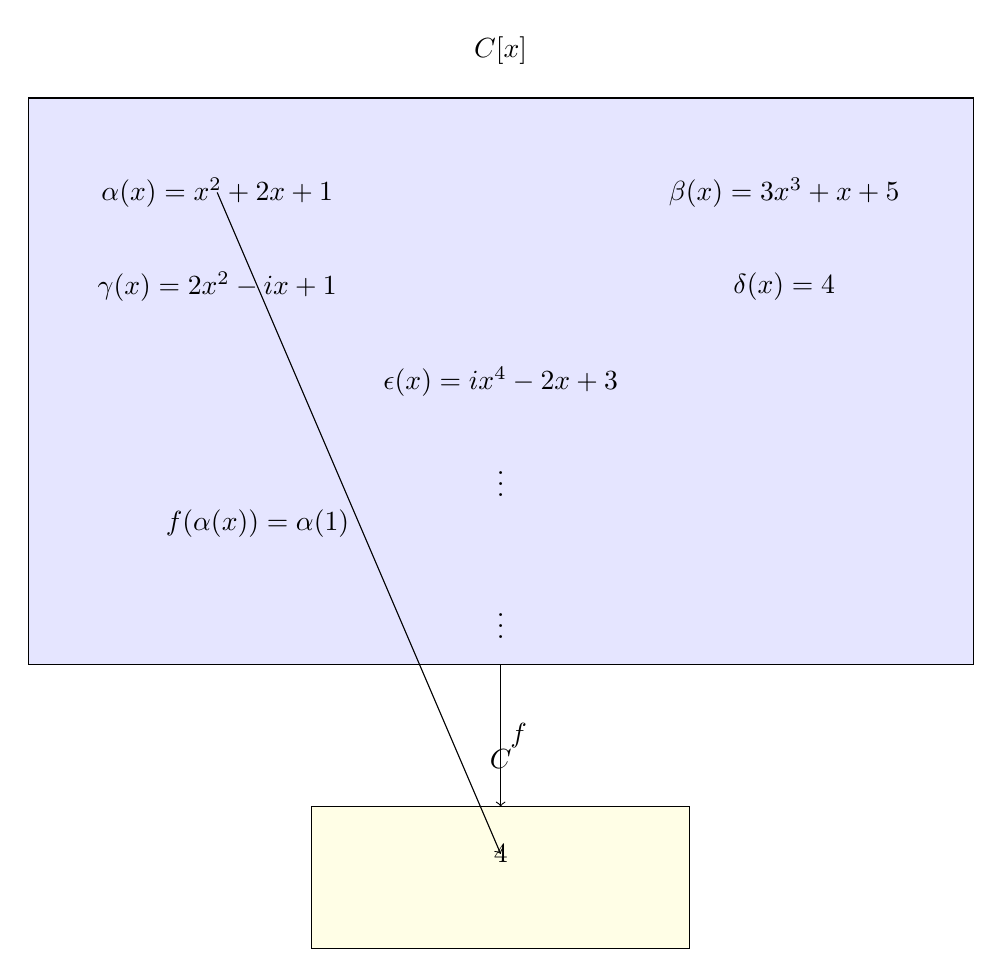
\begin{tikzpicture}[scale=1.2]
	% Draw the box for C[x]
	\draw[fill=blue!10] (0,0) rectangle (10,6);
	\node at (5,6.5) {$\mathbb{C}[x]$};
	
	% Examples of polynomials inside the box
	\node at (2,5) {$\alpha(x) = x^2 + 2x + 1$};
	\node at (8,5) {$\beta(x) = 3x^3 + x + 5$};
	\node at (2,4) {$\gamma(x) = 2x^2 - ix + 1$};
	\node at (8,4) {$\delta(x) = 4$};
	\node at (5,3) {$\epsilon(x) = ix^4 - 2x + 3$};
	
	% Arrow to C
	\draw[->] (5,0) -- (5,-1.5) node[midway, right] {$f$};
	
	% C box and example
	\draw[fill=yellow!10] (3,-3) rectangle (7,-1.5);
	\node at (5,-1) {$\mathbb{C}$};
	\node at (5,-2) {$4$}; % Example output
	
	% An arrow from the specific polynomial to the output
	\draw[->] (2,5) -- (5,-2) node[midway, left] {$f(\alpha(x)) = \alpha(1)$};
	
	% Dots to indicate continuation
	\node at (5,2) {$\vdots$};
	\node at (5,0.5) {$\vdots$};
\end{tikzpicture}

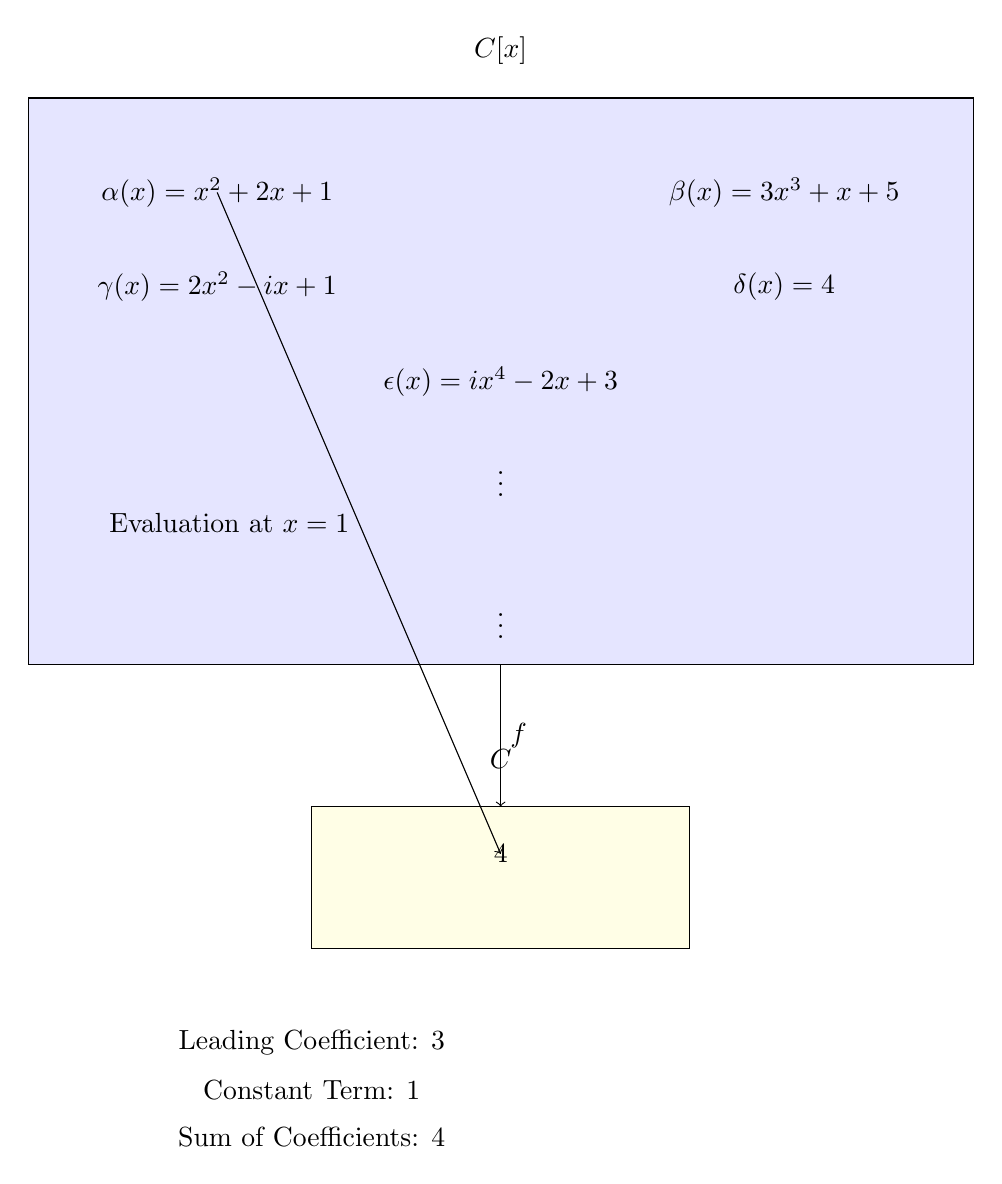
\begin{tikzpicture}[scale=1.2]
	% Draw the box for C[x]
	\draw[fill=blue!10] (0,0) rectangle (10,6);
	\node at (5,6.5) {$\mathbb{C}[x]$};
	
	% Examples of polynomials inside the box
	\node at (2,5) {$\alpha(x) = x^2 + 2x + 1$};
	\node at (8,5) {$\beta(x) = 3x^3 + x + 5$};
	\node at (2,4) {$\gamma(x) = 2x^2 - ix + 1$};
	\node at (8,4) {$\delta(x) = 4$};
	\node at (5,3) {$\epsilon(x) = ix^4 - 2x + 3$};
	
	% Arrow to C
	\draw[->] (5,0) -- (5,-1.5) node[midway, right] {$f$};
	
	% C box and example
	\draw[fill=yellow!10] (3,-3) rectangle (7,-1.5);
	\node at (5,-1) {$\mathbb{C}$};
	\node at (5,-2) {$4$}; % Example output
	
	% An arrow from the specific polynomial to the output
	\draw[->] (2,5) -- (5,-2) node[midway, left] {Evaluation at $x=1$};
	
	% Additional mappings
	\node at (3,-4) {Leading Coefficient: $3$};
	\node at (3,-4.5) {Constant Term: $1$};
	\node at (3,-5) {Sum of Coefficients: $4$};
	
	% Dots to indicate continuation
	\node at (5,2) {$\vdots$};
	\node at (5,0.5) {$\vdots$};
\end{tikzpicture}

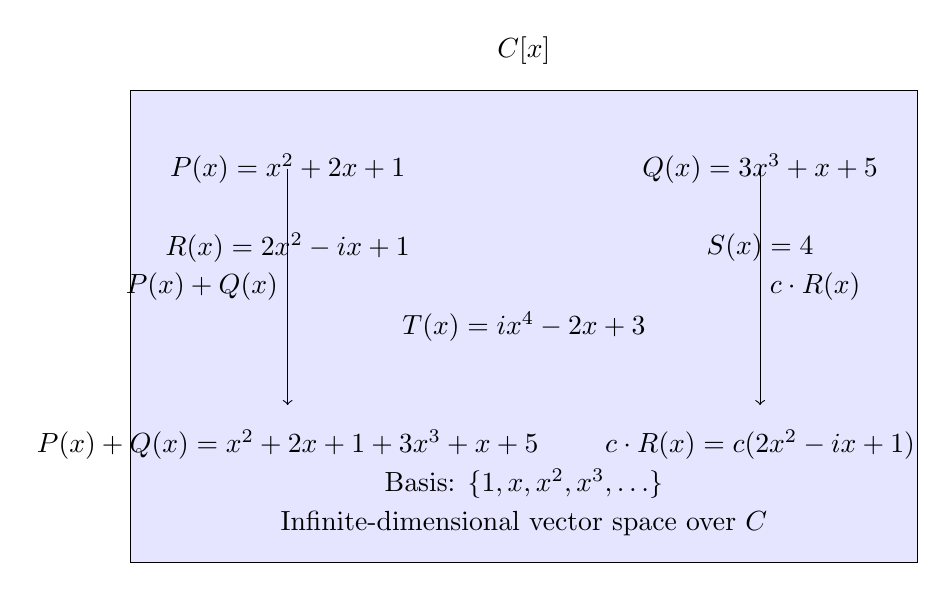
\begin{tikzpicture}
	% Draw the box for C[x]
	\draw[fill=blue!10] (0,0) rectangle (10,6);
	\node at (5,6.5) {$\mathbb{C}[x]$};
	
	% Examples of polynomials inside the box
	\node at (2,5) {$P(x) = x^2 + 2x + 1$};
	\node at (8,5) {$Q(x) = 3x^3 + x + 5$};
	\node at (2,4) {$R(x) = 2x^2 - ix + 1$};
	\node at (8,4) {$S(x) = 4$};
	\node at (5,3) {$T(x) = ix^4 - 2x + 3$};
	
	% Arrows indicating operations
	\draw[->] (2,5) -- (2,2) node[midway, left] {$P(x) + Q(x)$};
	\node at (2,1.5) {$P(x) + Q(x) = x^2 + 2x + 1 + 3x^3 + x + 5$};
	
	\draw[->] (8,5) -- (8,2) node[midway, right] {$c \cdot R(x)$};
	\node at (8,1.5) {$c \cdot R(x) = c(2x^2 - ix + 1)$};
	
	% Basis example
	\node at (5,1) {Basis: $\{1, x, x^2, x^3, \ldots\}$};
	\node at (5,0.5) {Infinite-dimensional vector space over $\mathbb{C}$};
\end{tikzpicture}


\section{Zorn's Lemma and Basis}
\subsection{Relations}
Let $\mathcal{R}\subseteq A\times A$ be a relation on a set $A$.
\begin{table}[h!]\setstretch{1.5}\adjustbox{scale=.7, center}{
\begin{tabular}{|c|c|c|c|}
	\hline
	\textbf{Property Type} & \textbf{Condition} & \textbf{Definition}& \textbf{Example} \\
	\hline
	\multirow{4}{*}{\textbf{Reflexive Properties}} 
	& Reflexive & $\forall a \in A, \ (a, a) \in R$ & Equality relation on $\mathbb{R}$ \\
	\cline{2-4}
	& Coreflexive & $\forall a, b \in A, \ (a, b) \in R \Rightarrow a = b$ & Identity relation $\{(a, a) : a \in A\}$ \\
	\cline{2-4}
	& Irreflexive (Anti-reflexive) & $\forall a \in A, \ (a, a) \notin R$ & "Is less than" relation on $\mathbb{R}$ \\
	\cline{2-4}
	& Non-Reflexive & $\exists a \in A, \ (a, a) \notin R$ & ``Is a friend of'' relation \\
	\hline
	\multirow{4}{*}{\textbf{Symmetric Properties}} 
	& Symmetric & $\forall a, b \in A, \ (a, b) \in R \Rightarrow (b, a) \in R$ & Equality relation on $\mathbb{R}$ \\
	\cline{2-4}
	& Asymmetric & $\forall a, b \in A, \ (a, b) \in R \Rightarrow (b, a) \notin R$ & ``Is parent of'' relation \\
	\cline{2-4}
	& Anti-Symmetric & $\forall a, b \in A, \ (a, b) \in R \ \text{and} \ (b, a) \in R \Rightarrow a = b$ & "Is less than or equal to" relation on $\mathbb{R}$ \\
	\cline{2-4}
	& Non-Symmetric & $\exists a, b \in A, \ (a, b) \in R \ \text{and} \ (b, a) \notin R \ \text{or} \ (a, b) \notin R \ \text{and} \ (b, a) \in R$ & "Is sibling of" relation\\
	\hline
	\multirow{3}{*}{\textbf{Transitive Properties}} 
	& Transitive & $\forall a, b, c \in A, \ (a, b) \in R \ \text{and} \ (b, c) \in R \Rightarrow (a, c) \in R$ & Divisibility relation on $\mathbb{N}$ \\
	\cline{2-4}
	& Anti-Transitive & $\forall a, b, c \in A, \ (a, b) \in R \ \text{and} \ (b, c) \in R \Rightarrow (a, c) \notin R$ & Hard to find simple example \\
	\cline{2-4}
	& Non-Transitive & $\exists a, b, c \in A, \ (a, b) \in R \ \text{and} \ (b, c) \in R \ \text{and} \ (a, c) \notin R$ & ``Is a friend of'' \\
	\hline
\end{tabular}}
\caption{Conditions and Examples for Relation Properties}
\end{table}

\begin{center}
\begin{figure}[h!]
	\centering
	\begin{subfigure}[t]{0.3\textwidth}
		\centering
		\begin{tikzpicture}[scale=1, >=Stealth, node distance=2.5cm, thick, main/.style = {draw, circle}]
		% Define styles
		\tikzset{
			reflexive/.style={->, loop, looseness=12, in=120, out=60, red},
			symmetric/.style={->, blue, bend left},
			transitive/.style={->, green!75!black}
		}
		
		% Nodes
		\node[main] (a) at (0,0) {a};
		\node[main] (b) [right of=a] {b};
		\node[main] (c) at (1.25,-2.5) {c};
		
		% Reflexivity
		\draw[reflexive] (a) to (a);
		\draw[reflexive] (b) to (b);
		\draw[reflexive] (c) to (c);
		\end{tikzpicture}
		\caption{Reflexive}
		\label{fig:reflexive}
	\end{subfigure}\hfill
	\begin{subfigure}[t]{0.3\textwidth}
		\centering
		\begin{tikzpicture}[scale=1, >=Stealth, node distance=2.5cm, thick, main/.style = {draw, circle}]
			% Define styles
			\tikzset{
				reflexive/.style={->, loop, looseness=12, in=120, out=60, red},
				symmetric/.style={->, blue, bend left},
				transitive/.style={->, green!75!black}
			}
			
			% Nodes
			\node[main] (a) at (0,0) {a};
			\node[main] (b) [right of=a] {b};
			\node[main] (c) at (1.25,-2.5) {c};
			
			% Reflexivity
			\draw[dotted, ->, red, bend left] (a) to (b);
			\draw[-, red, bend right] (a) to node[midway, below] {$a=b$} (b);
			%		\draw[reflexive] (c) to (c);
		\end{tikzpicture}
		\caption{Co-reflexive.}
		\label{fig:coreflexive}
	\end{subfigure}\hfill
	\begin{subfigure}[t]{0.3\textwidth}
		\centering
		\begin{tikzpicture}[scale=1, >=Stealth, node distance=2.5cm, thick, main/.style = {draw, circle}]
			% Define styles
			\tikzset{
				reflexive/.style={->, loop, looseness=12, in=120, out=60, red},
				symmetric/.style={->, blue, bend left},
				transitive/.style={->, green!75!black}
			}
			
			% Nodes
			\node[main] (a) at (0,0) {a};
			\node[main] (b) [right of=a] {b};
			\node[main] (c) at (1.25,-2.5) {c};
			
			% Reflexivity
			\draw[reflexive] (a) to node[] {\xmark} (a);
			\draw[reflexive] (b) to node[] {\xmark} (b);
			\draw[reflexive] (c) to node[] {\xmark} (c);
		\end{tikzpicture}
		\caption{Irreflexive}
		\label{fig:irreflexive}
	\end{subfigure}
	\caption{Reflexivity}
	\label{fig:reflexivity}
\end{figure}

\end{center}

\begin{center}
\begin{figure}[h!]
	\centering
	\begin{subfigure}[t]{0.3\textwidth}
		\centering
		\begin{tikzpicture}[scale=1, >=Stealth, node distance=2.5cm, thick, main/.style = {draw, circle}]
			% Define styles
			\tikzset{
				reflexive/.style={->, loop, looseness=12, in=120, out=60, red},
				symmetric/.style={->, blue, bend left},
				transitive/.style={->, green!75!black}
			}
			
			% Nodes
			\node[main] (a) at (0,0) {a};
			\node[main] (b) [right of=a] {b};
			\node[main] (c) at (1.25,-2.5) {c};
			
			% Reflexivity
			\draw[reflexive] (a) to (a);
			\draw[reflexive] (b) to (b);
			\draw[reflexive] (c) to (c);
		\end{tikzpicture}
		\caption{Reflexive}
		\label{fig:reflexive}
	\end{subfigure}\hfill
	\begin{subfigure}[t]{0.3\textwidth}
		\centering
		\begin{tikzpicture}[scale=1, >=Stealth, node distance=2.5cm, thick, main/.style = {draw, circle}]
			% Define styles
			\tikzset{
				reflexive/.style={->, loop, looseness=12, in=120, out=60, red},
				symmetric/.style={->, blue, bend left},
				transitive/.style={->, green!75!black}
			}
			
			% Nodes
			\node[main] (a) at (0,0) {a};
			\node[main] (b) [right of=a] {b};
			\node[main] (c) at (1.25,-2.5) {c};
			
			% Reflexivity
			\draw[dotted, ->, red, bend left] (a) to (b);
			\draw[-, red, bend right] (a) to node[midway, below] {$a=b$} (b);
			%		\draw[reflexive] (c) to (c);
		\end{tikzpicture}
		\caption{Co-reflexive.}
		\label{fig:coreflexive}
	\end{subfigure}\hfill
	\begin{subfigure}[t]{0.3\textwidth}
		\centering
		\begin{tikzpicture}[scale=1, >=Stealth, node distance=2.5cm, thick, main/.style = {draw, circle}]
			% Define styles
			\tikzset{
				reflexive/.style={->, loop, looseness=12, in=120, out=60, red},
				symmetric/.style={->, blue, bend left},
				transitive/.style={->, green!75!black}
			}
			
			% Nodes
			\node[main] (a) at (0,0) {a};
			\node[main] (b) [right of=a] {b};
			\node[main] (c) at (1.25,-2.5) {c};
			
			% Reflexivity
			\draw[reflexive] (a) to node[] {\xmark} (a);
			\draw[reflexive] (b) to node[] {\xmark} (b);
			\draw[reflexive] (c) to node[] {\xmark} (c);
		\end{tikzpicture}
		\caption{Irreflexive}
		\label{fig:irreflexive}
	\end{subfigure}
	\caption{Reflexivity}
	\label{fig:reflexivity}
\end{figure}
\end{center}

\begin{tikzpicture}[-Stealth]
	% Root node
%	\draw (-8,4) rectangle (8,-8);
	\node[centered] (set) at (0,3) {\large Non-empty Set $S\neq\emptyset$};
	\node[centered] (bi-op) at (0,1.5) {\large Binary Operation ($*$)};
	\node[centered] (magma) at (0,0) {\large Magma};
	
	% First level
	\node[centered] (semi) at (-6,-2.5) {\large Semi-group};
	\node[centered] (unital) at (0,-2.5) {\large Unital Magma};
	\node[centered] (quasi) at (6,-2.5) {\large Quasi-group};
	
	% Second level 
	\node[centered] (monoid) at (-6,-5) {\large Monoid};
	\node[centered] (asso-quasi) at (0,-5) {\large Associative Quasi-group};
	\node[centered] (loop) at (6,-5) {\large Loop};
	
	% Third level of subsets
	\node[centered] (group) at (0,-7.5) {\large Group};
	
	% Level 1
	\draw (set) -- (bi-op) node[] {};
	\draw (bi-op) -- (magma) node[] {};
	\draw (magma) -- (semi) node[midway, above left] {associativity};
	\draw (magma) -- (quasi) node[midway, above right] {divisibility};
	\draw (magma) -- (unital) node[] {};
	
	% Level 2
	\draw (semi) -- (monoid) node[midway] {identity};
	\draw (semi) -- (asso-quasi) node[] {};
	\draw (quasi) -- (loop) node[midway] {identity};
	\draw (quasi) -- (asso-quasi) node[] {};
	\draw (unital) -- (monoid) node[] {};
	\draw (unital) -- (loop) node[] {};
	
	% Level 3
	\draw (monoid) -- (group) node[midway, below left] {invertibility};
	\draw (loop) -- (group) node[midway, below right] {associativity};
	\draw (asso-quasi) -- (group) node[] {};
\end{tikzpicture}